\documentclass[conference,letterpaper,10pt]{IEEEtran}
\usepackage[letterpaper,left=0.65in,right=0.65in,top=0.7in,bottom=0.7in]{geometry}
\usepackage{amsmath,amssymb}
\usepackage{graphicx}
\usepackage{booktabs}
\usepackage{multirow}
\usepackage{tikz}
\usetikzlibrary{positioning,arrows.meta}
\usepackage{cite}
\usepackage{url}
\pagestyle{empty}

\title{PINN-Assisted Compact Modeling and Residual Diagnosis for TFT SPICE Simulation}

\author{
\IEEEauthorblockN{
Yifan Yang\IEEEauthorrefmark{1}\IEEEauthorrefmark{2},
Xiao Peng\IEEEauthorrefmark{1}\IEEEauthorrefmark{2},
Yunhe Li\IEEEauthorrefmark{2},
Zikang Mei\IEEEauthorrefmark{2},
and Wei Tang\IEEEauthorrefmark{2}\IEEEauthorrefmark{3}}
\IEEEauthorblockA{\IEEEauthorrefmark{2}Shanghai Jiao Tong University, Shanghai, China\\
\IEEEauthorrefmark{1}Equal contribution: v1o2058@sjtu.edu.cn, px.126666@sjtu.edu.cn\\
\IEEEauthorrefmark{3}Corresponding author: terry\_tang@sjtu.edu.cn}
}

\begin{document}
\maketitle
\thispagestyle{empty}

\begin{abstract}
Thin-film transistor (TFT) compact models are needed for SPICE simulation, but parameter extraction across device dimensions is difficult with limited geometries. This work presents a compact-model-centered PINN-assisted workflow for TFT modeling. A Verilog-A-compatible compact model is implemented in Python and checked against ngspice simulation. Conventional compact fitting establishes the measured-device baseline, and width/length holdout tests expose the limitation of traditional geometry scaling for the smallest channel length. A parameter PINN learns the mapping from device geometry to compact-model parameters, reducing the difficult \(80/10~\mu\mathrm{m}\) holdout error from \(1.54\) to \(0.47\) decade. A residual PINN then identifies bias regions where structured error remains. The results support a practical role for PINNs in TFT SPICE modeling: assisting parameter extraction, improving difficult geometry extrapolation, and guiding compact-model refinement.
\end{abstract}

\begin{IEEEkeywords}
thin-film transistor, compact model, SPICE, PINN, residual modeling, Verilog-A
\end{IEEEkeywords}

\section{Introduction}
Compact models connect device characterization to circuit simulation and remain central to TFT-based circuit design \cite{lu2018review,nagel1975spice2}. For emerging TFT technologies, the available dataset is often small: a few device geometries, repeated measurements, and several bias sweeps. Independent fits can reproduce measured curves, but circuit design needs a single SPICE-compatible description that remains useful across geometry and bias.

This paper studies a compact-model-centered workflow for three measured TFT geometries, denoted by channel width/length pairs \(80/10\), \(80/20\), and \(80/40~\mu\mathrm{m}\). The workflow follows the idea of physics-informed neural networks, where neural models are constrained or guided by physical or model structure \cite{raissi2019physics}. Here, the compact model remains the simulation layer, while neural modules are used for parameter mapping and residual diagnosis.

The contributions are threefold. First, a SPICE-compatible TFT compact model is implemented in both Python and Verilog-A/ngspice, and the two implementations are checked for numerical consistency. Second, compact fitting and holdout experiments separate measured-device fitting accuracy from geometry extrapolation accuracy. Third, parameter PINN and residual PINN modules are evaluated around the compact model for geometry-dependent parameter mapping and residual diagnosis.

\section{Modeling Workflow}
The drain current is described by a Verilog-A-compatible compact expression with threshold voltage, current prefactor, mobility-shape exponent, subthreshold factor, channel-length modulation, saturation scale, and off-current terms. The same equations are implemented in Python for fitting and checked against ngspice simulation \cite{ngspice_manual}.

The measured dataset contains output curves \(I_D\)-\(V_D\) and transfer curves \(I_D\)-\(V_G\) for the three geometries. The loss is evaluated in log-current space,
\begin{equation}
    \mathcal{L}_{I} = \frac{1}{N}\sum_i
    \left|\log_{10}(I_{D,i}^{\mathrm{fit}}+I_0)
    - \log_{10}(I_{D,i}^{\mathrm{meas}}+I_0)\right|,
\end{equation}
where \(I_0\) is a small numerical floor.

Fig.~\ref{fig:workflow} summarizes the workflow. Conventional fitting extracts compact parameters directly. The parameter PINN maps \((\log W,\log L)\) to compact-model parameters with current loss and smoothness regularization. The residual PINN keeps the parameter-PINN current as a baseline and learns a bounded correction in log-current space,
\begin{equation}
    \log_{10} I_D^{\mathrm{res}} =
    \log_{10} I_D^{\mathrm{base}} +
    r_{\theta}(V_G,V_D,\log W,\log L).
\end{equation}
The residual model is used mainly for diagnosis: the spatial distribution of \(r_\theta\) indicates where the compact description leaves systematic error.

\begin{figure}[t]
\centering

\includegraphics[width=0.88\columnwidth]{figures/model.png}
\vspace{0.2mm}
\resizebox{0.82\columnwidth}{!}{%
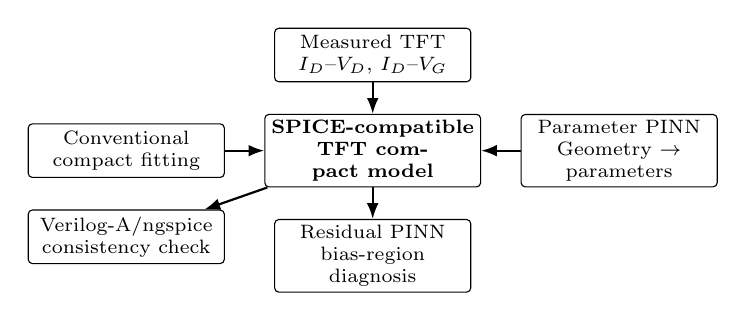
\begin{tikzpicture}[
    block/.style={
        draw,
        rounded corners=1.5pt,
        align=center,
        text width=2.35cm,
        minimum height=0.68cm,
        font=\scriptsize,
        inner sep=2pt
    },
    centerblock/.style={
        draw,
        rounded corners=1.5pt,
        align=center,
        text width=2.60cm,
        minimum height=0.76cm,
        font=\scriptsize\bfseries,
        inner sep=2pt
    },
    arrow/.style={-{Latex[length=2mm]}, thick}
]
\node[centerblock] (compact) {SPICE-compatible\\TFT compact model};
\node[block, above=4mm of compact] (data) {Measured TFT\\$I_D$--$V_D$, $I_D$--$V_G$};
\node[block, left=5mm of compact] (fit) {Conventional\\compact fitting};
\node[block, right=5mm of compact] (pinn) {Parameter PINN\\Geometry $\rightarrow$ parameters};
\node[block, below=4mm of compact] (res) {Residual PINN\\bias-region diagnosis};
\node[block, below=4mm of fit] (spice) {Verilog-A/ngspice\\consistency check};

\draw[arrow] (data) -- (compact);
\draw[arrow] (fit) -- (compact);
\draw[arrow] (pinn) -- (compact);
\draw[arrow] (compact) -- (res);
\draw[arrow] (compact) -- (spice);
\end{tikzpicture}%
}
\caption{Compact-model-centered workflow. Measured TFT structures are fitted with a SPICE-compatible compact model, then analyzed by parameter and residual PINN modules for geometry-dependent parameter mapping and bias-region diagnosis.}
\label{fig:workflow}
\end{figure}

\section{Results}
\subsection{Measured-device compact fitting}
Independent compact fitting gives mean absolute log errors of \(0.06\)--\(0.19\) decade on measured devices. The fitted Python model and Verilog-A/ngspice implementation agree to below \(10^{-3}\) decade on average, confirming transferability to the circuit simulator. This result establishes that the compact expression can describe the measured output and transfer curves when each geometry is fitted separately.

\subsection{Traditional width/length extrapolation}
The main difficulty appears in geometry extrapolation. A global conventional width/length fit gives a mean holdout error of \(1.54\) decade for the \(80/10~\mu\mathrm{m}\) device, while the other two holdout geometries remain below \(0.27\) decade. Enlarging the allowable subthreshold factor improves the measured-device fit; explicit source/drain resistance fitting gives no consistent gain for the present dataset.

\subsection{Parameter PINN for compact parameters}
The parameter PINN improves the difficult \(80/10~\mu\mathrm{m}\) holdout case. Table~\ref{tab:holdout} averages output and transfer errors for each held-out geometry. The \(80/10~\mu\mathrm{m}\) error is reduced from \(1.54\) to \(0.47\) decade, while the conventional fit remains competitive for the other two sizes.

\begin{table}[t]
\caption{Mean absolute log-current error in width/length holdout tests.}
\label{tab:holdout}
\centering
\begin{tabular}{lccc}
\toprule
Model & \(80/10\) & \(80/20\) & \(80/40\) \\
\midrule
Global compact fit & 1.543 & 0.213 & 0.269 \\
Parameter PINN & 0.467 & 0.337 & 0.314 \\
\bottomrule
\end{tabular}
\end{table}

\begin{figure}[t]
\centering

\includegraphics[width=0.72\linewidth]{figures/representative_80_10_holdout_idvd.png}
\caption{Representative \(80/10~\mu\mathrm{m}\) holdout curve at \(V_G=1\) V. The parameter PINN follows the measured output curve more closely than the global compact fit.}
\label{fig:wl}
\end{figure}

\subsection{Residual PINN for diagnosis}
The residual PINN is evaluated as a diagnostic and local-correction layer on top of the parameter-PINN baseline, and its results are reported separately from the width/length ranking in Table~\ref{tab:holdout}. It reduces the average pointwise holdout error for \(80/20\) and \(80/40~\mu\mathrm{m}\), and only slightly changes \(80/10~\mu\mathrm{m}\). For \(80/20~\mu\mathrm{m}\), the output-curve error decreases from \(0.172\) to \(0.091\) decade and the transfer-curve error from \(0.162\) to \(0.108\) decade.

\begin{figure}[t]
\centering
\begin{tabular}{cc}

\includegraphics[width=0.48\linewidth]{figures/residual_holdout_curve_reduction.png} &

\includegraphics[width=0.48\linewidth]{figures/residual_holdout_bias_heatmap.png}
\end{tabular}
\caption{Residual PINN diagnostics on holdout data. Positive values indicate lower log-current error after residual correction; local over-correction remains visible in selected subsets.}
\label{fig:residual}
\end{figure}

Bias-region analysis gives the clearest interpretation. Averaged over holdout devices, all regions except low-\(V_G\)/mid-\(V_D\) improve after residual correction. The strongest improvements occur in mid-\(V_G\)/mid-\(V_D\), mid-\(V_G\)/high-\(V_D\), and low-\(V_G\)/high-\(V_D\) regions. Device-resolved failures concentrate in high-\(V_G\)/mid-\(V_D\) output curves of \(80/10~\mu\mathrm{m}\), high-\(V_G\)/low-to-mid-\(V_D\) transfer curves of \(80/10~\mu\mathrm{m}\), and low-\(V_G\)/low-to-mid-\(V_D\) transfer curves of \(80/40~\mu\mathrm{m}\). These regions suggest possible missing descriptions in high-gate-bias linear operation, low-current transfer behavior, or geometry-dependent scaling.

\section{Conclusion}
A compact-model-centered PINN workflow was evaluated for TFT SPICE modeling with limited measured geometries. Conventional compact fitting provides accurate measured-device fits and simulator-compatible parameters, but width/length extrapolation can fail for the smallest channel length. A parameter PINN improves the difficult geometry holdout through smooth dimension-dependent compact parameters. A residual PINN maps remaining structured error and is best used as a diagnostic layer before conversion into explicit compact-model terms. Future work will extend the geometry set and test whether residual patterns can be translated into SPICE model terms for high-gate-bias and low-current operation. Processed data and paper-generation files are available at \url{https://github.com/Yang-Fran/tft-pinn-compact-modeling}.

\bibliographystyle{IEEEtran}
\bibliography{references}

\end{document}
